\documentclass[../main.tex]{subfiles}
\begin{document}

\section{Fundamentos teóricos}
En esta sección se abordan la teoría necesaria para comprender el enfoque propuesto en este trabajo. El objetivo principal es presentar los conceptos clave que sustentan el uso de técnicas de aprendizaje profundo en la segmentación semántica de lesiones de esclerosis múltiple a partir de imágenes de resonancia magnética.

Se comienza con una introducción a las redes neuronales convolucionales, que constituyen la base de los modelos empleados. A continuación, se describen las arquitecturas específicas utilizadas en este trabajo: U-Net y YOLO, ambas ampliamente reconocidas por su eficacia en tareas de segmentación. Posteriormente, se describe la segmentación semántica y finalmente se detalla la técnica de super-resolución mediante la red  FSRCNN, que se emplea como
estrategia de mejora de calidad de las imágenes de entrada. 

\subsection{Redes neuronales convolucionales}

Las redes neuronales convolucionales son una arquitectura especializada de redes profundas diseñada para procesar datos con estructura espacial, como las imágenes, que pueden interpretarse como una matriz bidimensional de píxeles. A diferencia de las redes densas tradicionales, las CNN explotan las propiedades locales de las imágenes mediante convoluciones, lo que las convierte en una herramienta muy eficaz para tareas como clasificación, detección y segmentación \cite{Alzubaidi2021}. En términos generales, una CNN se define por el uso de capas convolucionales, aunque su estructura concreta puede variar según la tarea: algunas incluyen capas totalmente conectadas al final (como en clasificación), mientras que otras son completamente convolucionales (como en segmentación o detección). Sus principales ventajas incluyen:

\begin{itemize}
    \item \textbf{Reducción de parámetros}: al reutilizar filtros a lo largo de la imagen, se disminuye significativamente el número de pesos, reduciendo el riesgo de sobreajuste y mejorando la eficiencia computacional.
    \item \textbf{Captura de relaciones espaciales locales}: los filtros pueden detectar patrones como bordes, texturas o formas, respetando la estructura espacial de los datos.
    \item \textbf{Invarianza a translaciones}: gracias a los pesos compartidos y operaciones de pooling, las CNN son robustas a pequeños desplazamientos y deformaciones en la imagen \cite{goodfellow2016deep}.
\end{itemize}

Una CNN está compuesta por una serie de capas que transforman progresivamente la imagen de entrada en una representación de alto nivel útil para la tarea objetivo. A continuación se describen sus componentes principales:

\begin{itemize}
    \item \textbf{Capa convolucional}: aplica filtros que recorren la imagen y generan mapas de activación. Cada filtro aprende a detectar una característica visual concreta.
    \item \textbf{Capa de activación}: normalmente se aplica una función como ReLU para introducir no linealidad y permitir el aprendizaje de relaciones complejas.
    \item \textbf{Capa de agrupamiento (pooling)}: reduce la dimensión espacial de los mapas de activación aplicando filtros (por ejemplo, de tamaño $2 \times 2$) con un cierto desplazamiento o \textit{stride} (habitualmente 2), conservando únicamente la información más relevante (como el valor máximo en cada región en el caso de \textit{max pooling}) y disminuyendo así la carga computacional.
    %\item \textbf{Capas totalmente conectadas (opcional)}: en tareas como clasificación, al final de la red los mapas se aplanan y se conectan a una red tradicional para producir la salida final (como una probabilidad por clase). Sin embargo, en tareas como segmentación o detección, las CNN pueden prescindir de estas capas y mantener una estructura completamente convolucional.
\end{itemize}

%\begin{figure}
%    \centering
%    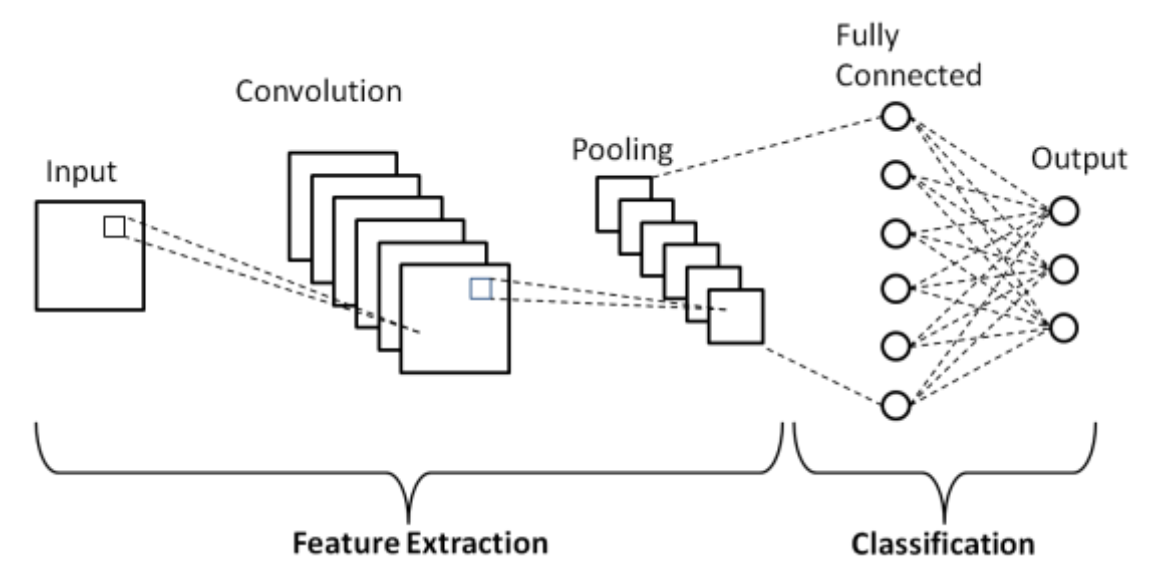
\includegraphics[width=\textwidth]{imgs/cnn-arquitectura.png}
%    \caption{Estructura básica de una red neuronal convolucional %(CNN) \cite{cnn_1}.}
%    \label{fig:cnn_arquitectura}
%\end{figure}

Las CNN aprenden representaciones jerárquicas: en las primeras capas se detectan patrones simples como bordes o texturas, mientras que en las capas más profundas se combinan esas representaciones para identificar estructuras más complejas y específicas de la tarea. Para lograr esto, las operaciones de convolución y agrupamiento son fundamentales. Como ejemplo ilustrativo, en la Figura~\ref{fig:cnn_bordes} se muestra cómo una CNN puede utilizar un filtro convolucional para detectar bordes verticales en una imagen en escala de grises. Este tipo de operación permite resaltar zonas donde se producen cambios bruscos de intensidad.

\begin{figure}
    \centering
    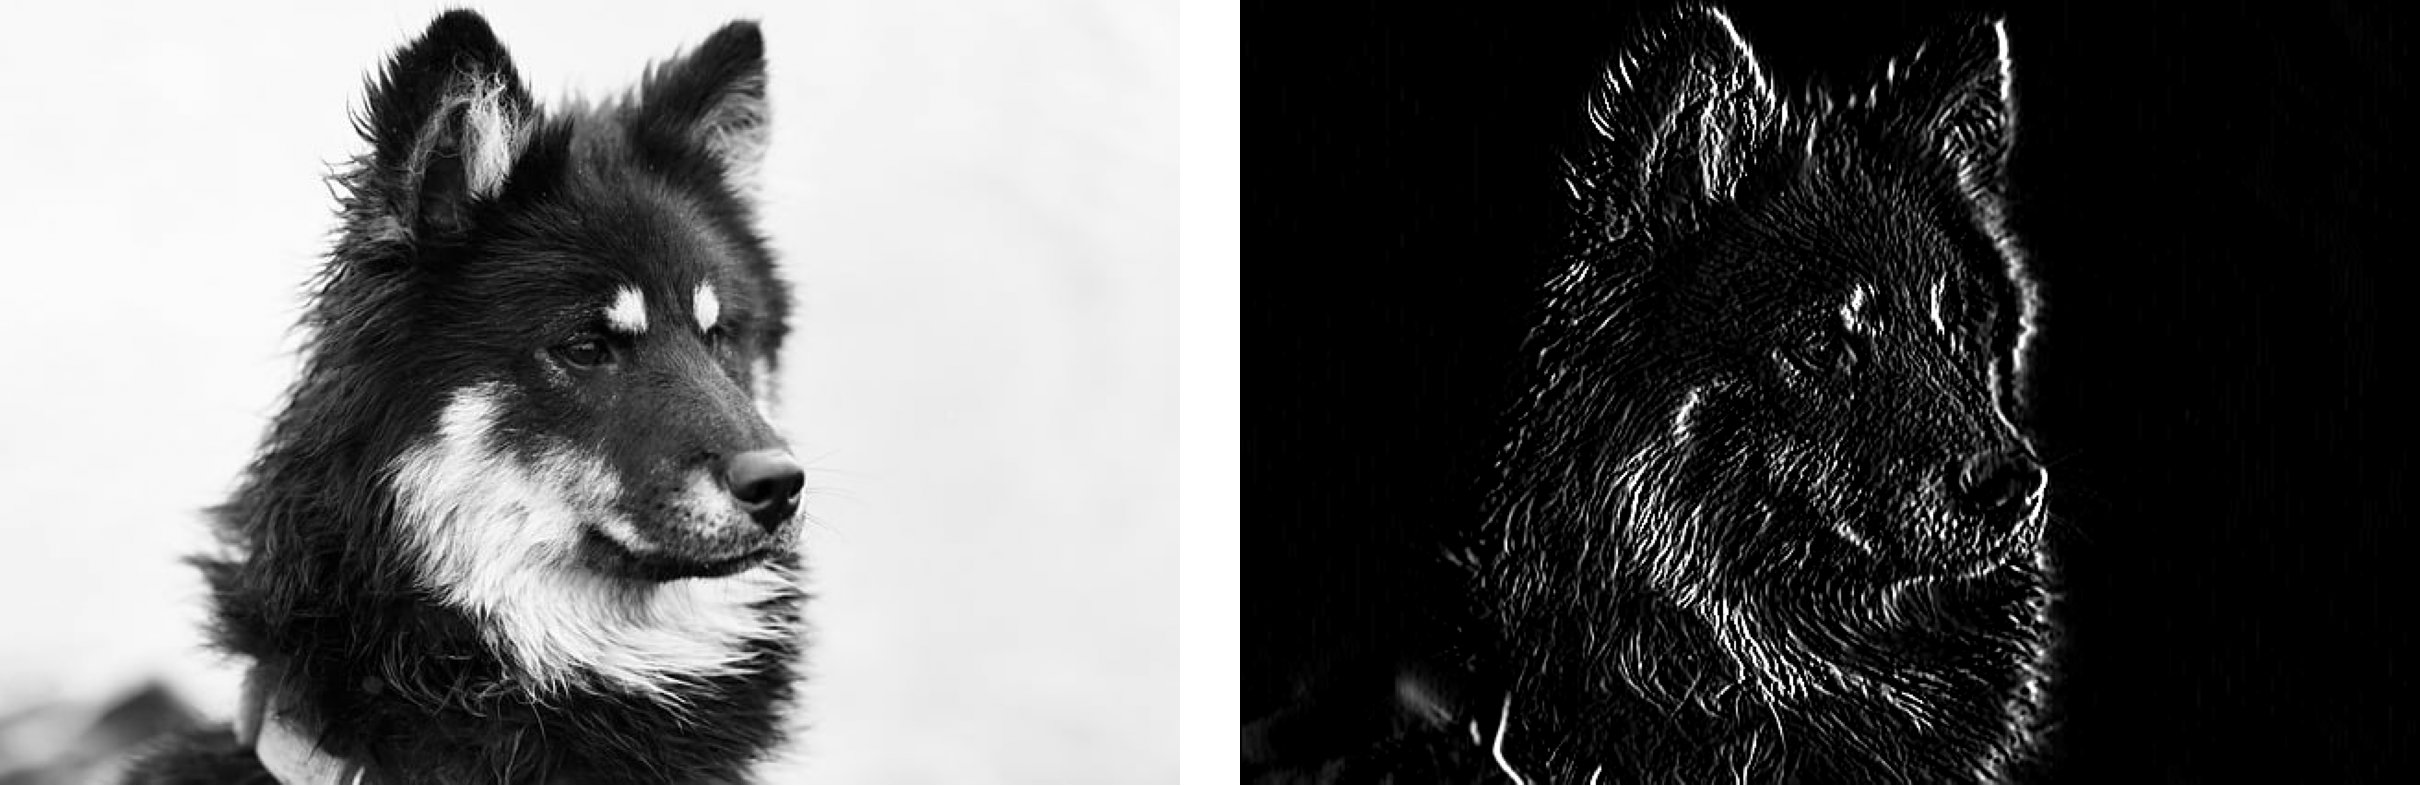
\includegraphics[width=\textwidth]{imgs/fundamentos/conv_operation.png}
    \caption{Ejemplo de operación de convolución con un filtro de detección de bordes (derecha) aplicado a una imagen original (izquierda).}
    \label{fig:cnn_bordes}
\end{figure}

La operación de agrupamiento, por su parte, tiene como objetivo principal disminuir el tamaño espacial (alto y ancho) de los mapas de activación (resultado obtenido tras la convolución), conservando la información más relevante. La Figura \ref{fig:con_operation} muestra la aplicación de la operación de agrupamiento, en este caso aplicando \textit{max pooling} sobre una matriz de entrada $4 \times 4$.

\begin{figure}
    \centering
    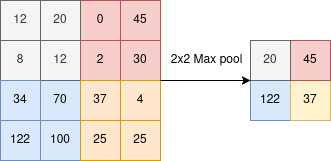
\includegraphics[width=0.5\linewidth]{imgs/fundamentos/max_pooling.drawio.png}
    \caption{Aplicación de la operación de agrupamiento en el caso de \textit{max pooling} con un filtro de tamaño $2 \times 2$ y un \textit{stride} de 2. A cada paso el filtro se mueve 2 posiciones en horizontal y vertical, calculando el valor máximo, lo que resulta en una matriz de dimensiones $2 \times 2$.}
    \label{fig:con_operation}
\end{figure}

\subsection{Segmentación semántica}
El uso más habitual de las CNN es la clasificación de imágenes, donde se asigna una única etiqueta a toda la imagen de entrada. Sin embargo, en muchas aplicaciones de visión por computador, especialmente en el ámbito médico, se requiere un nivel de detalle mucho mayor. En estos casos, no basta con conocer la presencia de una estructura, sino que es necesario localizarla con precisión. La segmentación semántica es la tarea de asignar a cada píxel una etiqueta de clase, es decir, particionar la imagen en subconjuntos mutuamente excluyentes, donde cada subconjunto delimita una región de interés de la imagen original \cite{HAO2020302}.

A diferencia de la detección de objetos —que emplea cajas delimitadoras— o la segmentación de instancias —que diferencia entre objetos individuales de una misma clase—, la segmentación semántica no distingue entre instancias, sino que clasifica cada píxel según la clase a la que pertenece. En la Figura \ref{fig:segmentacion_semantica} se puede observar un ejemplo de segmentación semántica.

\begin{figure}
    \centering
    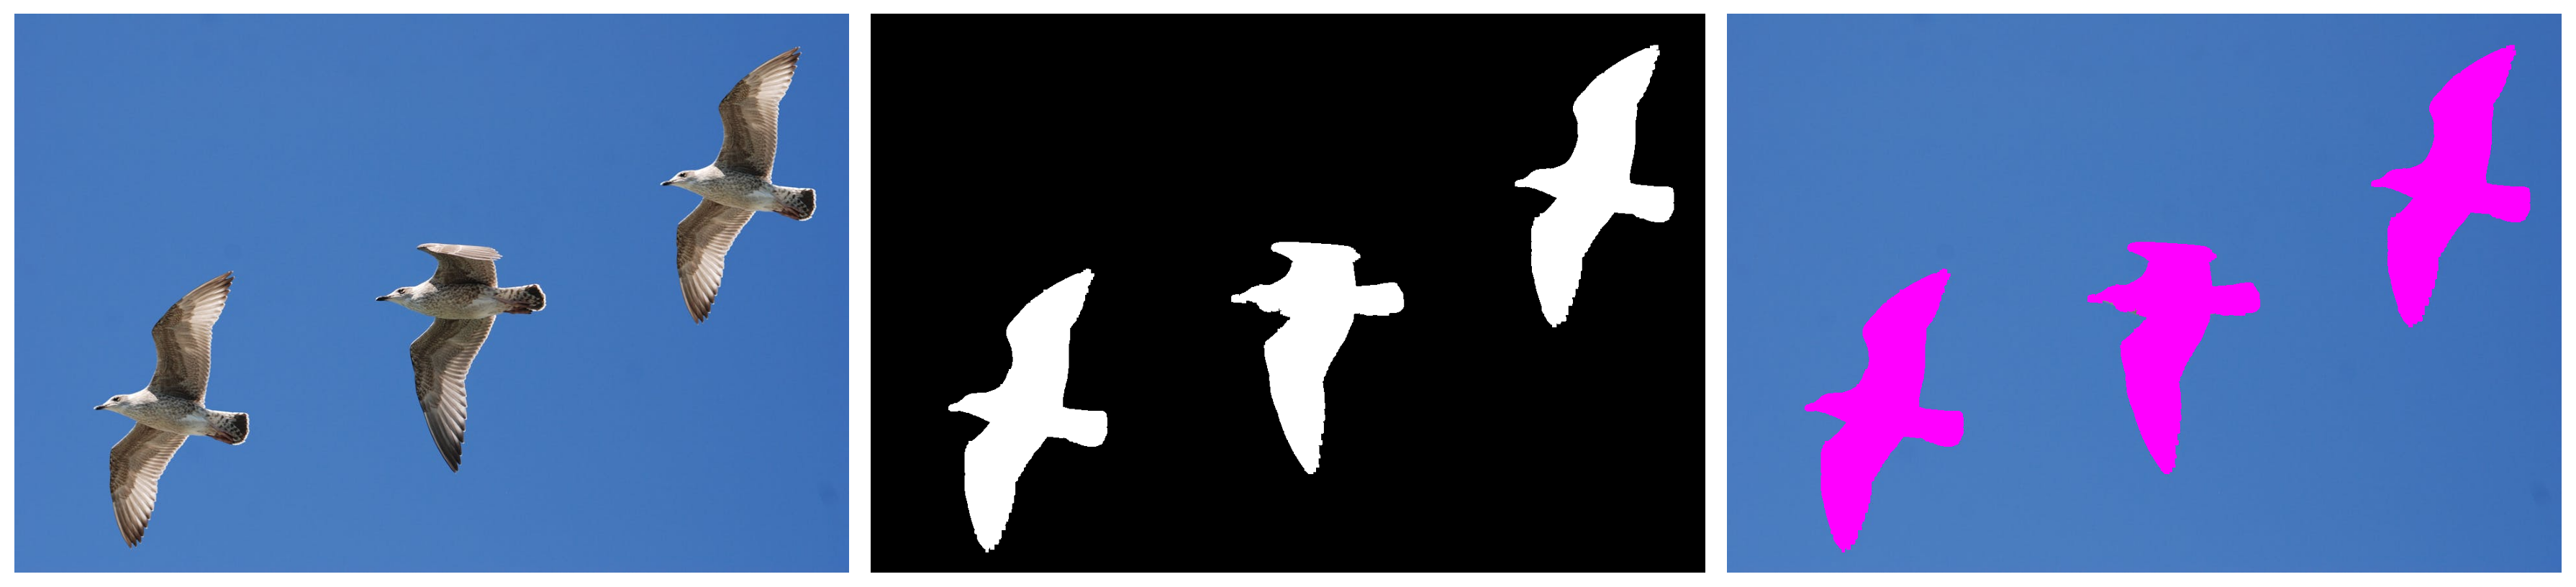
\includegraphics[width=0.7\linewidth]{imgs/fundamentos/segmentacion_semantica.png}
    \caption{Ejemplo de segmentación semántica sobre una imagen con gaviotas. De izquierda a derecha: imagen original, máscara generada a partir del contorno de las gaviotas y resultado final con superposición en color.}
    \label{fig:segmentacion_semantica}
\end{figure}

Este tipo de segmentación resulta esencial en tareas como la identificación de órganos, tejidos o lesiones patológicas en imágenes médicas, donde la precisión espacial es crítica para el diagnóstico y seguimiento clínico. En el caso particular de la esclerosis múltiple, la segmentación semántica permite detectar y cuantificar las lesiones de sustancia blanca presentes en la resonancia magnética, lo que puede facilitar el diagnóstico temprano y la evaluación de la progresión de la enfermedad. La Figura \ref{fig:segmentacion_mri} muestra un ejemplo de segmentación semántica con la red U-Net sobre la imagen MRI de un paciente con EM.

\begin{figure}
    \centering
    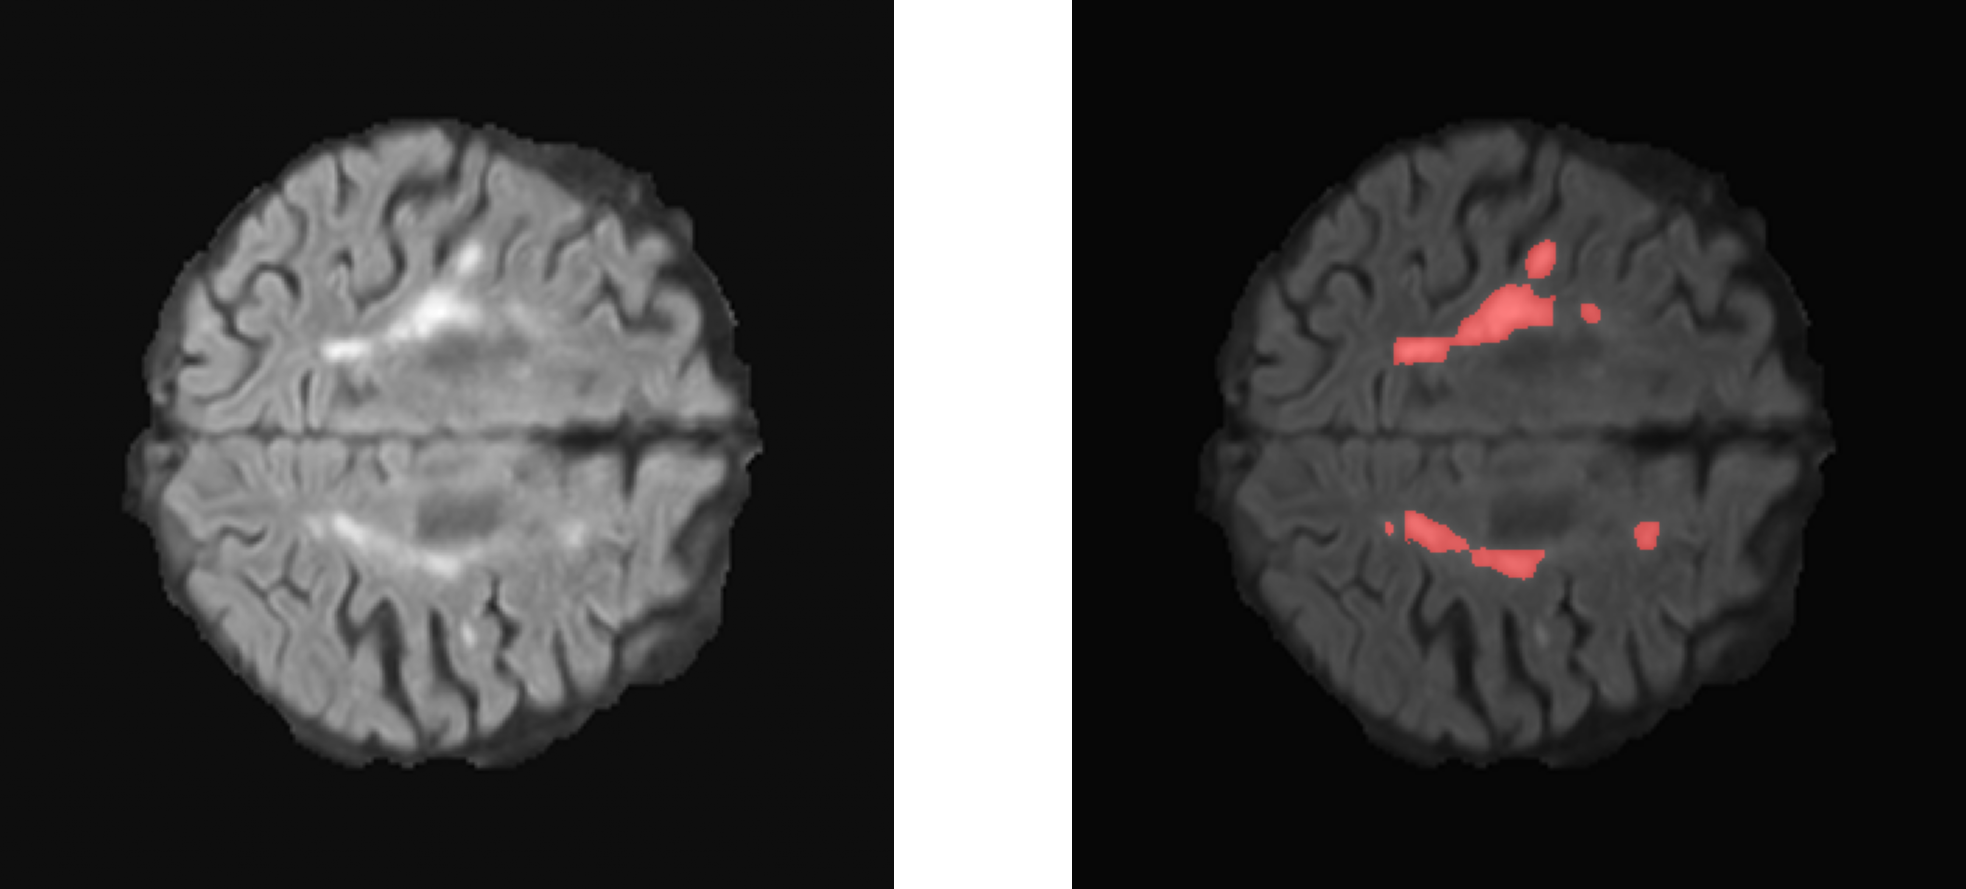
\includegraphics[width=0.7\linewidth]{imgs/fundamentos/segmentacion_mri.png}
    \caption{Ejemplo de segmentación semántica en una imagen de resonancia magnética cerebral. A la izquierda se muestra la imagen original en escala de grises. A la derecha, la misma imagen con la máscara de predicción superpuesta en color rojo, indicando las regiones identificadas automáticamente como posibles lesiones. La segmentación semántica permite clasificar cada píxel en función de su pertenencia a una categoría clínicamente relevante, facilitando el análisis estructural y la toma de decisiones diagnósticas.}
    \label{fig:segmentacion_mri}
\end{figure}

\subsection{U-Net}
U-Net es una arquitectura de CNN diseñada específicamente para tareas de segmentación semántica en imágenes biomédicas \cite{ronneberger2015unet}. A diferencia de los enfoques tradicionales basados en ventanas deslizantes, U-Net permite realizar predicciones a nivel de píxel sobre imágenes completas, ofreciendo alta precisión y eficiencia incluso con un número reducido de imágenes anotadas.

La arquitectura presenta una forma de \textit{U}, compuesta por un camino de contracción (\textit{contracting path}) y uno de expansión (\textit{expanding path}). El primero actúa como codificador, extrayendo características a distintas escalas mediante convoluciones seguidas de operaciones de \textit{max pooling}. El segundo realiza una decodificación progresiva mediante capas de \textit{up-convolution}, fusionando la información de baja resolución con las características de alta resolución obtenidas durante la fase de contracción. Esta estructura simétrica permite al modelo capturar tanto el contexto global como los detalles locales, esenciales para segmentar estructuras pequeñas o con bordes imprecisos.

\begin{figure}
    \centering
    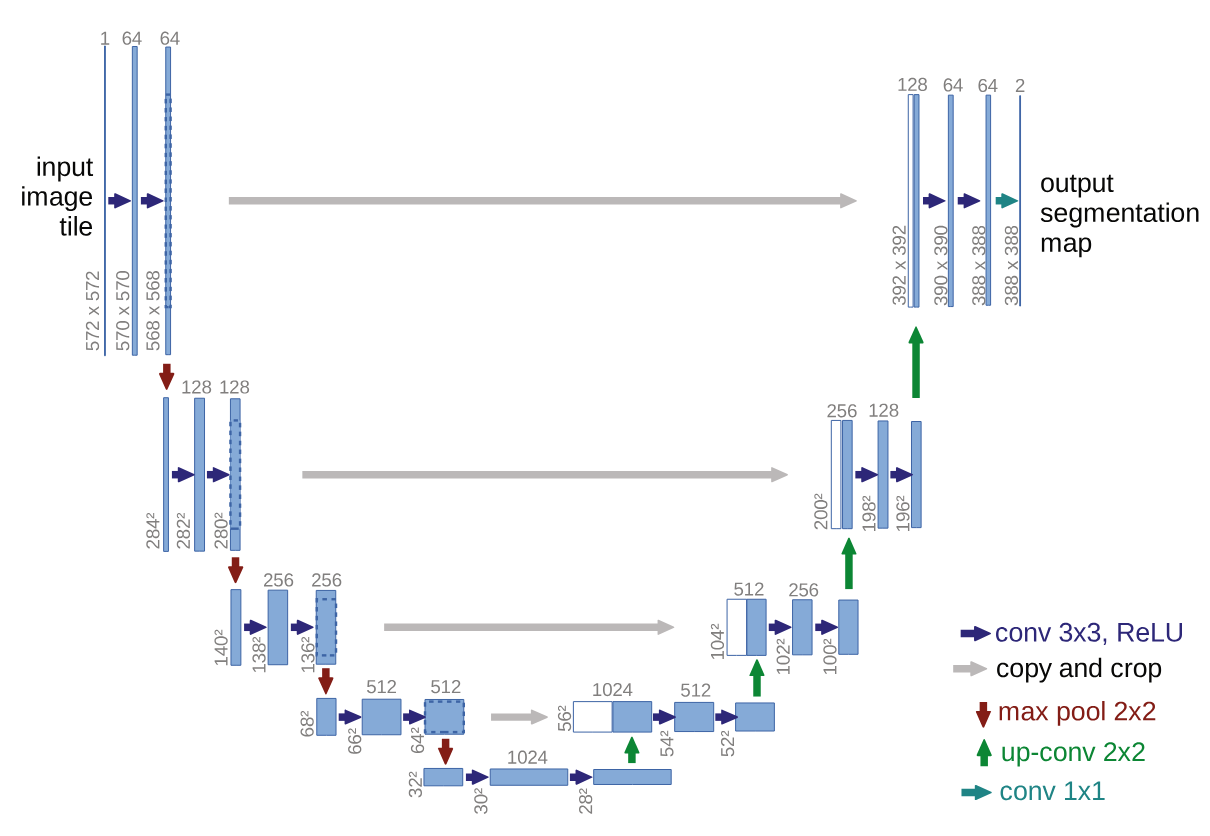
\includegraphics[width=\textwidth]{imgs/fundamentos/unet-estructura.png}
    \caption{Arquitectura de la red U-Net \cite{ronneberger2015unet}.}
    \label{fig:u-net-arquitectura}
\end{figure}

En la Figura~\ref{fig:u-net-arquitectura} se muestra la arquitectura de la U-Net, compuesta por un camino de contracción (izquierda) y otro de expansión simétrico (derecha). Cada bloque azul representa un mapa de características multicanal, con el número de canales indicado en la parte superior. Las dimensiones están indicadas en la parte inferior izquierda de cada bloque. Las operaciones incluyen convoluciones $3\times3$ con activación ReLU (azul oscuro), max pooling $2\times2$ (flechas rojas), up-convoluciones $2\times2$ (flechas verdes), y convoluciones $1\times1$ al final (verde azulado). Las flechas grises horizontales indican las conexiones por copia y recorte entre el encoder y el decoder, que permiten recuperar la información espacial de alta resolución.

\subsection{YOLO}

YOLO es un enfoque innovador para la detección de objetos que reformula el problema como una tarea de regresión directa, eliminando la necesidad de proponer regiones o aplicar clasificadores múltiples por separado. El modelo procesa toda la imagen de entrada con una única red neuronal convolucional, que predice simultáneamente las coordenadas de las cajas delimitadoras y las probabilidades de clase asociadas \cite{redmon2016lookonceunifiedrealtime}.

La imagen se divide en una cuadrícula de tamaño fijo, donde cada celda es responsable de predecir un número determinado de cajas delimitadoras ($B$) para los objetos cuyo centro caiga dentro de ella. Cada una de estas cajas se acompaña de una puntuación de confianza, calculada como el producto de la probabilidad de que haya un objeto y la coincidencia con el objeto real (IoU). Además, se predicen las probabilidades de clase para cada celda. La arquitectura general de YOLO, mostrada en la Figura~\ref{fig:yolo_arquitectura}, puede dividirse en tres bloques principales:

\begin{enumerate}
    \item \textbf{Entrada}: una imagen de tamaño fijo es introducida en la red.
    \item \textbf{Extracción de características}: la imagen atraviesa varias capas convolucionales y de pooling que permiten detectar patrones visuales progresivamente más complejos, desde bordes y texturas hasta formas completas.
    \item \textbf{Predicción}: las características extraídas alimentan una capa final que divide la imagen en una cuadrícula y predice, por cada celda, las cajas delimitadoras, sus puntuaciones de confianza y las probabilidades de clase.
\end{enumerate}

\begin{figure}[H]
    \centering
    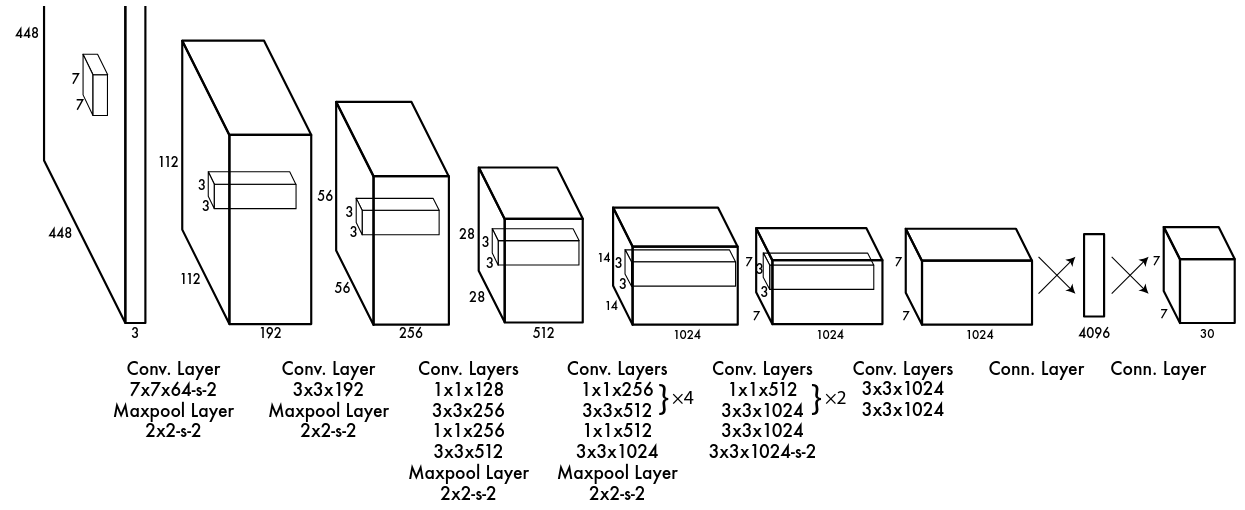
\includegraphics[width=0.7\linewidth]{imgs/fundamentos/yolo_arquitectura.png}
    \caption{Arquitectura general de YOLO. El modelo divide la imagen en una cuadrícula y predice simultáneamente cajas delimitadoras, puntuaciones de confianza y clases en una sola pasada, permitiendo detección en tiempo real \cite{yolo}.}
    \label{fig:yolo_arquitectura}
\end{figure}

Este enfoque unificado permite que YOLO logre detección de objetos en tiempo real con un buen equilibrio entre velocidad y precisión, lo que lo convierte en una arquitectura popular también en tareas de segmentación por detección, especialmente en contextos donde la eficiencia computacional es crítica.

\subsection{Super-resolución con FSRCNN}
La super-resolución es una técnica de procesamiento de imágenes cuyo objetivo es reconstruir una imagen de alta resolución (\textit{High Resolution} o HR, por sus siglas en inglés) a partir de una o varias imágenes de baja resolución (\textit{Low Resolution} o LR) \cite{sr_systematic_r}. En el contexto de imágenes médicas, esta tarea adquiere una gran relevancia, ya que una mayor resolución espacial puede mejorar la visualización de detalles anatómicos sutiles o pequeñas lesiones que podrían pasar desapercibidas. Tradicionalmente, la super-resolución se abordaba mediante métodos cómo la interpolación u otros ya mencionados, pero en los últimos años han cobrado protagonismo obteniendo mejores resultados los enfoques basados en aprendizaje profundo \cite{ANWAR_SR}. Estos modelos aprenden a mapear directamente las imágenes LR a HR mediante redes CNN.

Entre los modelos más representativos de super-resolución se encuentra FSRCNN (Fast Super-Resolution Convolutional Neural Network), una arquitectura propuesta por Dong et al.\cite{dong2016} (véase Figura \ref{fig:fsrcnn_arquitectura}), que mejora significativamente tanto la precisión como la velocidad de su predecesor, SRCNN (Super-Resolution 
Convolutional Neural Network). 

SRCNN realiza primero una interpolación bicúbica para escalar la imagen a la resolución deseada antes de procesarla. A continuación, aplica tres capas convolucionales que se encargan de extraer características locales, mapearlas de forma no lineal y reconstruir la imagen mejorada. Este enfoque presenta limitaciones en eficiencia y calidad debido a la interpolación inicial. FSRCNN, en cambio, introduce varias mejoras clave: elimina la necesidad de interpolación previa y trabaja directamente con la imagen en baja resolución. Su arquitectura incluye módulos para extraer características, reducir y expandir la dimensionalidad, aplicar múltiples capas de mapeo no lineal y, finalmente, realizar una deconvolución para generar la imagen en alta resolución. Este diseño permite obtener resultados más rápidos y precisos, mejorando tanto el rendimiento como la calidad final de la reconstrucción.

\begin{figure}
    \centering
    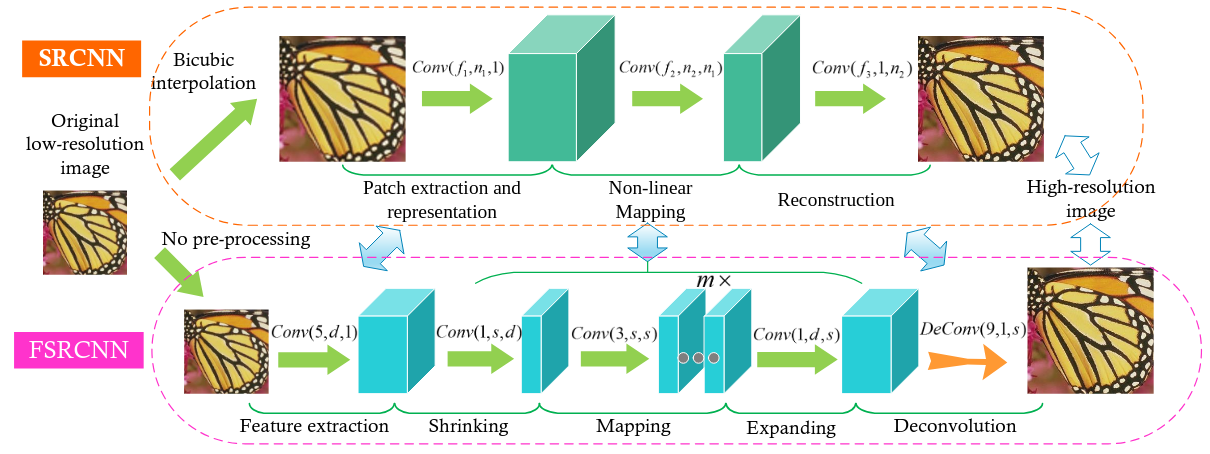
\includegraphics[width=0.7\linewidth]{imgs/fundamentos/fsrcnn_arquitectura.png}
    \caption{Comparación entre las arquitecturas de SRCNN y FSRCNN. SRCNN realiza una interpolación bicúbica previa y luego aplica tres capas convolucionales para extraer características y reconstruir la imagen. FSRCNN, por su parte, elimina la necesidad de preprocesamiento mediante interpolación y emplea una arquitectura optimizada con etapas de extracción, reducción y expansión de características, seguidas de una deconvolución final. Esta reorganización mejora tanto la precisión como la eficiencia computacional en tareas de super-resolución \cite{dong2016}.}
    \label{fig:fsrcnn_arquitectura}
\end{figure}

\end{document}